% !TeX TXS-program:compile = txs:///lualatex

\documentclass[a4paper,11pt]{article}
\usepackage[breakable]{cp-base}
\graphicspath{{./graphics/}}
%variables
\donnees[%
	typedoc=CHAPITRE~,numdoc=9,classe=1\up{ère} 2M2,matiere={[SPÉ.MATHS]},annee=2022,titre={Suites arithmétiques, géométriques}]

%formatage
\author{Pierquet}
\title{\nomfichier}
\hypersetup{pdfauthor={Pierquet},pdftitle={\nomfichier},allbordercolors=white,pdfborder=0 0 0,pdfstartview=FitH}
%divers
\lhead{\entete{\matiere}}
\chead{\entete{\lycee}}
\rhead{\entete{\classe{} - Chapitre \thepart}}
\lfoot{\pied{\matiere}}
\cfoot{\logolycee{}}
\rfoot{\pied{\numeropagetot}}

\begin{document}

\newcommand{\coord}[3]{\vect{#1}\begin{pmatrix}#2\\#3\end{pmatrix}}

\pagestyle{fancy}

\part{CH09 - Suites arithmétiques, géométriques}

\medskip

\begin{ccadre}
Ce chapitre porte sur l'étude de deux types de suites particulières : les suites arithmétiques et les suites géométriques. Ces suites ont la particularité de permettre de passer très facilement de la \textbf{formule de récurrence} à la \textbf{formule explicite} !
\end{ccadre}

\section{Suites arithmétiques}

\subsection{Définition}

\begin{cdefi}
Une suite $\suiten$ est dite \textbf{arithmétique} si l'on passe d'un terme au suivant en \textbf{ajoutant toujours le même nombre} $r$, appelé \textbf{raison} de la suite.

Autrement dit, une suite est \textbf{arithmétique} si sa formule de récurrence est du type : \[u_{n+1}=u_n+r\quad \mbox{ pour tout } n \pg 0.\]
\end{cdefi}

\begin{cexemple}
La suite des nombres impairs $1 - 3 - 5 - 7 - 9 - 11 - 13 - \ldots$ est arithmétique de raison 2.
\end{cexemple}

\begin{crmq}
Une suite pour laquelle on passe d'un terme au suivant en \textit{retranchant} toujours le même nombre est également arithmétique, mais sa raison est négative.

Ainsi, la suite $12 - 11,5 - 11 - 10,5 - 10 - 9,5 - \ldots$ est arithmétique de raison $-0,5$.
\end{crmq}

\begin{cmethode}
Pour démontrer qu'une suite est arithmétique :
\begin{itemize}
	\item soit on transcrit le texte de l'énoncé sous forme de formule de récurrence,
	\item soit on calcule la \textbf{différence} $u_{n+1}-u_n$ entre deux termes consécutifs et on montre que cette différence est constante et ne dépend pas de $n$.
	
	Le résultat de ce calcul est alors la \textbf{raison} $r$ de la suite.
\end{itemize}
\end{cmethode}

\begin{cexemple}
On va démontrer que la suite définie par $u_n=2n-3$ pour tout $n \pg 0$ est arithmétique.
\begin{itemize}
	\item on calcule $u_{n+1}$ : $u_{n+1}=2(n+1)-3=2n-1$ ;
	\item puis la différence : $u_{n+1}-u_n=(2n-1)-(2n-3)=-1+3=2$.
\end{itemize}
Le résultat ne dépend plus de $n$, donc la suite est \textbf{arithmétique} de raison $r=2$.
\end{cexemple}

\subsection{Formule explicite}

\begin{cprop}
Soit $\suiten$ une suite \textbf{arithmétique} de raison $r$ et de premier terme $u_0$. Alors : \[u_n=u_0+n\times r \quad  \text{ pour tout } n \in \N.\]
\end{cprop}

\begin{crmq}
Si le premier terme de la suite n'est pas $u_0$ mais $u_1$, on a la propriété : \[u_n=u_1+(n-1) \times r \quad \text{ pour tout }n \pg 1 \]%
et, pour n'importe quel rang $p$ : \[u_n=u_p+(n-p) \times r \quad \text{ pour tout } n \pg p.\]
\end{crmq}

\begin{cdemo}
$u_1=u_0+r$ ;

$u_2=u_1+r=u_0+r+r=u_0+2r$ ;

$u_3=u_2+r=u_0+2r+r=u_0+3r$ ;

$\vdots$

$u_n=u_{n-1}+r=u_0+(n-1) \times r +r = u_0 + n\times r$.
\end{cdemo}

\begin{cexemple}
Ma tirelire contient 23\,€. Au 1\ier janvier de cette année, j'ai décidé d'y mettre 5\,€ tous les mois. Quelle somme contiendra-t-elle à la fin de l'année ?
\begin{itemize}
	\item La suite $\suiten[t]$ où $t_n$ est la somme contenue dans la tirelire à la fin du $n$-ième mois d'économie est une suite arithmétique de raison $r=5$ et de premier terme $t_0=23$.
	\item À la fin de l'année, il y aura dans la tirelire $t_{12}=t_0+12 \times r=23+12 \times 5=83 $\,€.
\end{itemize}
\end{cexemple}

\subsection{Sens de variation}

\begin{cprop}
Une suite \textbf{arithmétique} est toujours \textbf{monotone}. Elle est \textbf{croissante} si sa \textbf{raison} est \textbf{positive}, et décroissante si sa raison est négative.
\end{cprop}

\begin{cdemo}
Pour étudier le sens de variation d'une suite, on étudie le signe de la différence $u_{n+1}-u_n$, et dans le cas d'une suite arithmétique, cette différence est égale à la raison $r$ !
\end{cdemo}

\subsection{Modélisation}

\begin{cprop}
Les points du nuage qui représente une suite $(u_n)$ \textbf{arithmétique} de raison $r$ sont tous \textbf{alignés}, sur la \textbf{droite} de coefficient directeur $r$ et d'ordonnée à l'origine $u_0$.
\begin{center}
	\tunits{0.5}{0.5}
	\tdefgrille{0}{10}{1}{1}{0}{8}{1}{1}
	\begin{tikzpicture}[x=\xunit cm,y=\yunit cm,>=latex]
		\tgrilles[line width=0.3pt,cyan!50] ;
		\axestikz*[width=1pt] ; \axextikz[width=1pt,tickwidth=3pt]{0,2,...,8} ;
		\foreach \x in {0,1,...,9} \draw[line width=1pt] (\x,3pt)--(\x,-3pt) ;
		\foreach \y in {0,1,...,7} \draw[line width=1pt] (3pt,\y)--(-3pt,\y) ;
		\foreach \i in {0,1,...,7}{
			\draw[line width=0.75pt,densely dotted,red!75,->] (\i,{2.5+0.5*\i}) -| ({\i+1},{2.5+\i*0.5+0.5});
			\draw[fill,red] (\i,{2.5+0.5*\i}) circle[radius=1.5pt] ({\i+1},{2.5+\i*0.5+0.5}) circle[radius=1.5pt];}
		\draw[red] (4,3.5) node {$r>0$} ;
	\end{tikzpicture}
\end{center}
\end{cprop}

\begin{cdemo}
Le point de coordonnée $(0\,;\,u_0)$ est bien un point du nuage, et pour une unité supplémentaire en abscisse (c'est-à-dire au rang d'après), les ordonnées augmentent de $r$ : on retrouve bien la définition du coefficient directeur d'une droite. On remarquera également la cohérence entre le sens de variation d'une fonction affine et celui d'une suite arithmétique\ldots
\end{cdemo}

\begin{cprop}
Les suites \textbf{arithmétiques} modélisent des évolutions successives à \textbf{accroissements constants}. On parle également dans ce cas d'\textbf{évolution linéaire}.
\end{cprop}

\subsection{Somme des premiers termes}

\begin{cthm}
Pour tout entier naturel $n$ non nul, \[1+2+3+ \dots + n=\frac{n(n+1)}{2}.\]
\end{cthm}

\begin{cdemo}
Notons $T_n=1+2+\dots+n$ qui est appelé nombre \textit{triangulaire}, on peut le représenter avec $T_n$ pions \og en triangle \fg{} :

\begin{center}%merci Anne ;-)	
	%nombre triangulaire T1
	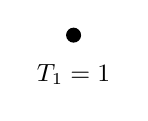
\begin{tikzpicture} [x=0.33cm,y=0.33cm,font=\small]
		\draw [fill] (0.,0.) circle (2.5pt);
		\draw (0,-1.5) node {$T_1=1$};
	\end{tikzpicture}
	\hspace{1cm}
	%nombre triangulaire T2
	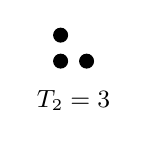
\begin{tikzpicture} [x=0.33cm,y=0.33cm,font=\small]
		\draw [fill] (0.,0.) circle (2.5pt);
		\draw [fill] (0.,1.) circle (2.5pt);
		\draw [fill] (1.,0.) circle (2.5pt);
		\draw (0.5,-1.5) node {$T_2=3$};
	\end{tikzpicture}
	\hspace{1cm}
	%nombre triangulaire T3
	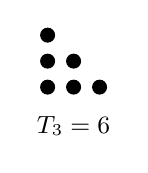
\begin{tikzpicture} [x=0.33cm,y=0.33cm,font=\small]
		\draw [fill] (0.,0.) circle (2.5pt);
		\draw [fill] (0.,1.) circle (2.5pt);
		\draw [fill] (1.,0.) circle (2.5pt);
		\draw [fill] (0.,2.) circle (2.5pt);
		\draw [fill] (1.,1.) circle (2.5pt);
		\draw [fill] (2.,0.) circle (2.5pt);
		\draw (1,-1.5) node {$T_3=6$};
	\end{tikzpicture}
	\hspace{1cm}	
	%nombre triangulaire T4
	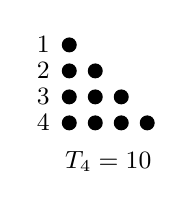
\begin{tikzpicture} [x=0.33cm,y=0.33cm,font=\small]
		\draw [fill] (0.,0.) circle (2.5pt);
		\draw [fill] (0.,1.) circle (2.5pt);
		\draw [fill] (1.,0.) circle (2.5pt);
		\draw [fill] (0.,2.) circle (2.5pt);
		\draw [fill] (1.,1.) circle (2.5pt);
		\draw [fill] (2.,0.) circle (2.5pt);
		\draw [fill] (3.,0.) circle (2.5pt);
		\draw [fill] (2.,1.) circle (2.5pt);
		\draw [fill] (1.,2.) circle (2.5pt);
		\draw [fill] (0.,3.) circle (2.5pt);
		\draw (-1,3) node {1};
		\draw (-1,2) node {2};
		\draw (-1,1) node {3};
		\draw (-1,0) node {4};
		\draw (1.5,-1.5) node {$T_4=10$};
	\end{tikzpicture}
	\hspace{1cm}
	% nombre triangulaire Tn
	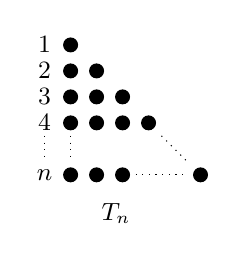
\begin{tikzpicture} [x=0.33cm,y=0.33cm,font=\small]
		\draw [fill] (0.,0.) circle (2.5pt);
		\draw [fill] (0.,1.) circle (2.5pt);
		\draw [fill] (1.,0.) circle (2.5pt);
		\draw [fill] (0.,2.) circle (2.5pt);
		\draw [fill] (1.,1.) circle (2.5pt);
		\draw [fill] (2.,0.) circle (2.5pt);
		\draw [fill] (3.,0.) circle (2.5pt);
		\draw [fill] (2.,1.) circle (2.5pt);
		\draw [fill] (1.,2.) circle (2.5pt);
		\draw [fill] (0.,3.) circle (2.5pt);
		\draw (-1,3) node {1};
		\draw (-1,2) node {2};
		\draw (-1,1) node {3};
		\draw (-1,0) node {4};
		\draw (-1,-2) node {$n$};
		\draw [dotted] (-1.,-0.5) -- (-1.,-1.5);
		\draw [dotted] (0.,-0.5) -- (0.,-1.5);
		\draw [dotted] (2.5,-2) -- (4.5,-2);
		\draw [dotted] (3.5,-0.5) -- (4.5,-1.5);
		\draw [fill] (0.,-2.) circle (2.5pt);
		\draw [fill] (1.,-2.) circle (2.5pt);
		\draw [fill] (2.,-2.) circle (2.5pt);
		\draw [fill] (5.,-2.) circle (2.5pt);
		\draw (1.75,-3.5) node {$T_n$};
	\end{tikzpicture}
\end{center}

En juxtaposant deux triangles identiques, l'un avec des pions noirs et l'autre avec des blancs, on obtient des rectangles :
\begin{itemize}
	\item le rectangle formé avec $2 \times T_n$ pions est formé de $n$ lignes et $n+1$ colonnes (1 avec que des pions noirs et $n$ qui commencent par un pion blanc)  ;
	\item le rectangle contient donc $n(n+1)$ pions ;
	\item ainsi, $2 \times T_n=n(n+1)$.
\end{itemize}

\begin{center}
	%rectangle  T3 *2
	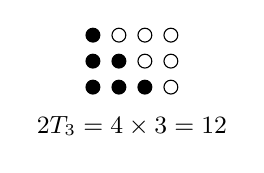
\begin{tikzpicture} [x=0.33cm,y=0.33cm,font=\small]
		\draw [fill] (0.,0.) circle (2.5pt); 
		\draw [fill] (0.,1.) circle (2.5pt);
		\draw [fill] (1.,0.) circle (2.5pt);
		\draw [fill] (0.,2.) circle (2.5pt);
		\draw [fill] (1.,1.) circle (2.5pt);
		\draw [fill] (2.,0.) circle (2.5pt);
		\draw (1,2) circle (2.5pt);
		\draw (2,1) circle (2.5pt);
		\draw (2,2) circle (2.5pt);
		\draw (3,0) circle (2.5pt);
		\draw (3,1) circle (2.5pt);
		\draw (3,2) circle (2.5pt);
		\draw (1.5,-1.5) node {$2T_3=4 \times 3=12$};
	\end{tikzpicture}
	\hspace{1cm}	
	% rectangle Tn*2
	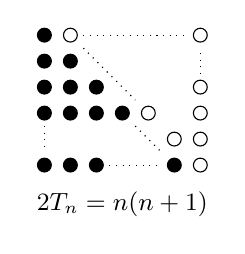
\begin{tikzpicture} [x=0.33cm,y=0.33cm,font=\small]
		\draw [fill] (0.,0.) circle (2.5pt);
		\draw [fill] (0.,1.) circle (2.5pt);
		\draw [fill] (1.,0.) circle (2.5pt);
		\draw [fill] (0.,2.) circle (2.5pt);
		\draw [fill] (1.,1.) circle (2.5pt);
		\draw [fill] (2.,0.) circle (2.5pt);
		\draw [fill] (3.,0.) circle (2.5pt);
		\draw [fill] (2.,1.) circle (2.5pt);
		\draw [fill] (1.,2.) circle (2.5pt);
		\draw [fill] (0.,3.) circle (2.5pt);
		\draw [dotted] (0.,-0.5) -- (0.,-1.5);
		\draw [dotted] (2.5,-2) -- (4.5,-2);
		\draw [dotted] (3.5,-0.5) -- (4.5,-1.5);
		\draw [fill] (0.,-2.) circle (2.5pt);
		\draw [fill] (1.,-2.) circle (2.5pt);
		\draw [fill] (2.,-2.) circle (2.5pt);
		\draw [fill] (5.,-2.) circle (2.5pt);
		\draw (6,-2) circle (2.5pt);
		\draw (6,-1) circle (2.5pt);
		\draw (5,-1) circle (2.5pt);
		\draw (6,0) circle (2.5pt);
		\draw (4,0) circle (2.5pt);
		\draw (6,1) circle (2.5pt);
		\draw (1,3) circle (2.5pt);
		\draw (6,3) circle (2.5pt);
		\draw [dotted] (6,1.5) -- (6,2.5);
		\draw [dotted] (1.5,3) -- (5.5,3);
		\draw [dotted] (1.5,2.5) -- (3.5,0.5);
		\draw (3,-3.5) node {$2T_n=n(n+1)$};
	\end{tikzpicture}
\end{center}
\end{cdemo}

\begin{cprop}
La \textbf{somme} des premiers termes d'une suite \textbf{arithmétique} est égale à :\[\text{nombre de termes} \times \frac{\text{premier terme + dernier terme}}{2}.\]%
Autrement dit, \[u_0+u_1+\dots+u_n=(n+1)\times \frac{u_0+u_n}{2}.\]
\end{cprop}

\pagebreak

\begin{cdemo}
On a :
\vspace{-5pt}
\begin{flalign*}
	u_0+u_1+u_2+\dots+u_n &= u_0+(u_0+r)+(u_0+2r)+\dots+(u_0+nr)& \\
	&= (u_0+ \dots +u_0)+r(1+2+\dots+n) \\
	&= (n+1)u_0+r \times \frac{n(n+1)}{2} \\
	&= (n+1)\left(u_0+\frac{rn}{2}\right) \\
	&= (n+1) \left( \frac{u_0+u_0+rn}{2} \right) \\
	&= (n+1)\times \frac{u_0+u_n}{2}
\end{flalign*}
\end{cdemo}

\section{Suites géométriques}

\subsection{Définition}

\begin{cdefi}
Une suite $\suiten$ est dite \textbf{géométrique} si l'on passe d'un terme au suivant en \textbf{multipliant toujours par le même nombre} $q$, appelé ici aussi \textbf{raison} de la suite.

Autrement dit, une suite est \textbf{géométrique} si sa formule de récurrence est du type : \[u_{n+1}=u_n \times q \quad \text{ pour tout } n \pg 0.\]
\end{cdefi}

\begin{cexemple}
La suite des puissances de dix : $1-10-100-1000-10000-\ldots$ est géométrique de raison 10.
\end{cexemple}

\begin{crmq}
Une suite pour laquelle on passe d'un terme au suivant en divisant toujours par le même nombre est également géométrique, puisque diviser par un nombre revient à multiplier par son inverse.
\end{crmq}

\begin{cmethode}
Pour démontrer qu'une suite est géométrique :
\begin{itemize}
	\item soit on transcrit le texte de l'énoncé sous forme de formule de récurrence ;
	\item soit on calcule le \textbf{quotient} $\dfrac{u_{n+1}}{u_n}$ entre deux termes consécutifs et on montre que ce quotient est constant et ne dépend pas de $n$.
	
	Le résultat de ce calcul est alors la \textbf{raison} $q$ de la suite.
\end{itemize}
\end{cmethode}

\begin{cexemple}
On souhaite démontrer que la suite définie par $u_n=5\times 3^n$ pour tout $n \pg 0$ est géométrique.
\begin{itemize}
	\item on calcule $u_{n+1}$ : $u_{n+1}=5\times 3^{n+1}=5 \times 3^n \times 3$ ;
	\item puis le quotient $\frac{u_{n+1}}{u_n}=\frac{5 \times 3^n \times 3}{5\times 3^{n}}=3$.
\end{itemize}
Le résultat ne dépend plus de $n$, donc la suite est \textbf{géométrique} de raison $q=3$.
\end{cexemple}

\subsection{Formule explicite}

\begin{cprop}
Soit $\suiten$ une suite \textbf{géométrique} de raison $q$ et de premier terme $u_0$.

Alors on a :\[u_n=u_0\times q^n \quad  \text{ pour tout } n \in \N.\]
\end{cprop}

\begin{crmq}
Si le premier terme de la suite n'est pas $u_0$ mais $u_1$, on a la propriété : \[u_n=u_1 \times q^{n-1} \quad \text{ pour tout }n \pg 1\]%
et, pour n'importe quel rang $p$ : \[u_n=u_p \times q^{n-p} \quad \text{ pour tout }n \pg p.\]
\end{crmq}

\begin{cdemo}
$u_1=u_0\times q$

$u_2=u_1 \times q=u_0  \times q\times q=u_0\times q^2$

$u_3=u_2 \times q =u_0 \times q^2 \times q =u_0 \times q^3$

$\vdots$

$u_n=u_{n-1} \times q=u_0 \times q^{n-1}\times q = u_0 \times q^n$.
\end{cdemo}

\begin{cexemple}
Je place en banque une somme de 350\,€. Au 1\ier janvier de chaque année, je perçois sur mon compte des intérêts qui s'élèvent à 3\,\% de la somme placée pendant l'année écoulée.  Quelle somme sera disponible sur mon compte au bout de 5 ans ?
\begin{itemize}
	\item Au bout d'un an, il y aura $350+\frac{3}{100}\times 350=350+10,5=360,5$\,€.
	\item Au bout de deux ans, il y aura $306,5+\frac{3}{100}\times 360,5=360,5+10,815 \approx 371,31 $\,€.
	\item La suite $\suiten[c]$ où $c_n$ est la somme placée à la fin de la $n$-ième année est une suite géométrique de raison $q=1,03$ et de premier terme $c_0=350$.
	
	En effet, $c_{n+1}=c_n+\frac{3}{100} \times c_n=c_n+0,03c_n=1,03c_n$. 
	\item Au bout de 5 ans, il y aura donc sur le compte $c_{5}=c_0 \times q^ 5 = 350 \times 1,03^ 5 \approx 405,75 $\,€.
\end{itemize}
\end{cexemple}

\subsection{Sens de variation}

\begin{cprop}
Une suite \textbf{géométrique} n'est pas toujours monotone. Soit $q$ un réel :
\begin{itemize}
	\item La suite ($q^n$) est \textbf{croissante} si $q>1$.
	\item La suite ($q^n$) est \textbf{décroissante} si $0<q<1$.
	\item La suite ($q^n$) est \textbf{non monotone} si $q<0$.
\end{itemize}
\end{cprop}

\begin{cdemo}
On a $q^{n+1} -q^{n} = q^{n} \times q - q^{n}=q^{n} (q-1)$.

Le signe de ce produit dépend donc du signe de $q$ et de $q-1$.
\end{cdemo}

\subsection{Modélisation}

\begin{cprop}
Les suites \textbf{géométriques} modélisent des évolutions successives à \textbf{taux constant}. On parle également dans ce cas d'\textbf{évolution exponentielle}.
\end{cprop}

\begin{crmq}
On utilisera notamment une suite géométrique pour modéliser toute augmentation ou diminution d'un \textbf{pourcentage} constant. En effet, une quantité qui augmente de $t$ \% est multipliée par $CM=1+\frac{t}{100}$.
\end{crmq}

\subsection{Somme des premiers termes}

\begin{cthm}
Pour tout $q \neq 1$ et tout entier naturel $n$ non nul, \[1+q+q^2+q^3+ \dots + q^n=\frac{1-q^{n+1}}{1-q}.\]
\end{cthm}

\begin{cdemo}
On a :

$(1+q+q^2+q^3+ \dots + q^n)(1-q)=1-q+q-q^2+q^2-q^3+\dots+q^n-q^{n+1}=1-q^{n+1} $ donc on obtient le résultat voulu en divisant les deux membres par $1-q$ qui est non nul.
\end{cdemo}

\begin{cprop}
La \textbf{somme} des premiers termes d'une suite \textbf{géométrique} est égale à :\[ \text{premier terme} \times \frac{1 - \text{raison}^{\text{nombre de termes}}}{1 - \text{raison} }.\]%
Autrement dit, \[u_0+u_1+ \dots + u_n=u_0 \times \frac{1-q^{n+1}}{1-q}.\]
\end{cprop}

\begin{cdemo}
On a :

$u_0+u_1+u_2+\dots+u_n = u_0+(u_0 \times q)+(u_0\times q^2)+\dots+(u_0 \times q^n) = u_0(1+q+q^2+ \dots + q^n)$.
\end{cdemo}

\begin{cexercice}
Une puce se déplace sur le dos d'un âne. Son premier saut a une longueur de 40~mm. À cause de la fatigue, chacun de ses sauts a une longueur égale à la moitié de la longueur du saut précédent.

On note $\suiten_{n \pg 1}$ la suite des longueurs des sauts de cette puce.
\begin{enumerate}
	\item Quelle est la nature de la suite $(u_n)$ ?
	\item Combien mesure le huitième saut de la puce ?
	\item Quelle est la distance totale parcourue par la puce au bout des 8 premiers sauts ?
	%\item On suppose qu'au départ, la puce est au niveau de la croupe de l'âne.  \`A votre avis, au bout de combien de sauts arrivera-t-elle sur la tête de l'animal ? Argumentez.
\end{enumerate}
\end{cexercice}

\end{document}